\documentclass[12pt]{article}

\usepackage{fullpage}
\usepackage{graphicx, rotating, booktabs} 
\usepackage{times} 
\usepackage{natbib} 
\usepackage{indentfirst} 
\usepackage{setspace}
\usepackage{grffile} 
\usepackage{hyperref}
\usepackage{adjustbox}
\usepackage{amsmath}
\setcitestyle{aysep{}}


\singlespace
\title{\textbf{Alliance Participation and Military Spending}}
\author{Joshua Alley\footnote{Graduate Student,
Department of Political Science, Texas A\&M University.}}
\date{{\normalsize \today}}

\bibliographystyle{apsr}

\begin{document}

\maketitle 

\doublespace 

\begin{abstract}
How does alliance participation affect military spending? 
Some argue that joining an alliance increases defense expenditures, while others contend that it produces spending cuts.
I argue both views are correct under certain conditions; how alliance participation affects growth in military expenditures depends on treaty scope and state capability. 
Highly capable major powers use alliances and military spending to increase their influence in international relations. 
Alliance participation usually increases major power military spending, but expenditure growth is lower in broad treaties.
Less capable non-major powers focus on immediate security. 
Though alliance participation usually decreases non-major power military spending, growth is higher in broad treaties. 
Treaty scope modifies the impact of alliance participation through formal issue linkages because broad treaties cover many issues and circumstances. 
I test the argument by creating a measure of alliance treaty scope and employing it in a multilevel model. 
The research design generates new empirical evidence linking alliance participation and growth in state military spending from 1816 to 2007. 
I find that greater treaty scope increases growth in military spending from alliance participation in non-major powers and decreases spending growth for major powers.  
These results help scholars and policymakers better understand a central question about alliance politics that has been debated in scholarship for decades. 
\end{abstract}


 \newpage 


\section{Introduction}


Scholars of international relations have long acknowledged that there are two ways for states to increase their security. 
States can invest in indigenous military capability or form alliances.\footnote{\cite{Morgenthau1948, Altfield1984, Morrow1993}}
Because both policies provide security, broadly defined, alliance participation should change how states invest in military capability. 
But exactly how alliances influence military spending remains unclear. 


Existing scholarship produces contrary predictions and evidence on the question of alliance participation and military spending. 
One view, which I call the \textit{force multiplier perspective}, expects alliance participation will reduce military spending.\footnote{\cite{Morrow1993, Conybeare1994, DigiuseppePoast2016}} 
The other view, which I label the \textit{foreign entanglement perspective}, predicts alliance participants will spend more on defense.\footnote{\cite{Diehl1994, MorganPalmer2006}}
This paper addresses the divide by explaining when alliance participation leads to more or less defense spending. 
In doing so, it helps clarify a longstanding debate about alliance politics.


Debate between the force multiplier and foreign entanglement perspectives largely ignores heterogeneity among alliances, which is essential to alliance politics scholarship.\footnote{\cite{Morrow1991, Leeds2003, LeedsAnac2005, Fordham2010, Mattes2012, Benson2012, Poast2013, Johnsonetal2015}}  
Given differences between treaties and states, alliance participation could plausibly increase or decrease defense expenditures. 
I use state capability and treaty scope to explain how alliance treaty participation impacts military spending. 


Major powers use alliances and military spending to increase their influence--- shaping international relations to match their interests.
Joining alliances usually increases major power growth in military spending, as these states require more capability to support their commitments abroad. 
Non-major powers, by contrast, use alliances and defense expenditures to ensure their territorial security.
Because alliances provide extra security without forcing these countries to protect others, alliance participation often reduces non-major power growth in military spending. 
Changes in treaty scope alter the consequences of alliance participation for major and non-major powers, however. 


Treaties with broad scope address many circumstances and issues.
Broad alliances cover multiple issues beyond core commitments of military intervention, including extra defense cooperation, forming international organizations, or improving economic ties.  
For example, a 1992 defense treaty between Uzbekistan and Kazakhstan promises military aid, non-military cooperation and most-favored nation status. 


Broad treaties add to major power influence and constrain non-major power freedom of action through issue-linkages. 
Thus, although alliance participation usually increases major power military spending, growth is lower in broad treaties compared to growth in narrower alliances.  
Conversely, while alliance participation usually decreases non-major power military spending, growth is higher in broad treaties relative to more narrow agreements.


I employ a novel research design to test my argument.
First, I develop a latent measure of alliance treaty scope. 
I then incorporate that measure into a multilevel model which estimates how alliance treaty characteristics modify the impact of alliance participation on growth in military spending.
To capture differences in state capability, I fit the model on separate samples of major and non-major power states from 1816 to 2007. 
I find that expanding treaty scope increases the impact of alliance participation on growth in non-major power military spending.
I also find that greater treaty scope reduces the impact of alliance participation on growth in major power military spending. 


My argument and findings suggest that major and non-major powers face different tradeoffs in alliance politics.
Broad commitments give major powers more influence, but increase entanglement abroad.
For non-major powers, broad treaties provide more benefits at the cost of freedom to reduce military spending. 


These tradeoffs illuminate two salient issues in US foreign policy. 
First, treaty scope is relevant to debates between advocates of deep engagement\footnote{\cite{Brooksetal2013}} and restraint\footnote{\cite{Posen2014}} in grand strategy about the value of US alliances. 
Advocates of restraint argue that low allied defense spending requires excessive US military spending, so the US should withdraw many of its alliances.
Proponents of deep engagement believe the benefits of alliance participation exceed the costs. 
While my argument gives a partial accounting of alliance costs and benefits, it suggests issue linkages can address low allied defense spending without withdrawing from a treaty.  


Second, debates about ``free-riding'' by US allies should consider the limited formal scope of most US treaties. 
US allies are able to spend less on defense because the United States offers narrow alliances. 
While limits on treaty scope limit entanglement abroad, they also constrain US influence to demand more military expenditures. 


The paper proceeds as follows. 
First, I summarize competing arguments and empirical evidence on alliance participation and military spending. 
Then I describe my argument in more detail. 
The third and fourth sections present the research design and results. 
The final section concludes with a discussion of the results and implications for scholarship and policy.  



\section{Force Multiplier or Foreign Entanglement?}


% quick intro and straight into it
Scholarship on alliance participation and military spending is divided between force multiplier and foreign entanglement views.
Each emphasizes one aspect of alliance politics throughout multiple arguments.  
I start with the substitution and public goods logics connecting alliance participation with reduced defense spending. 


\subsection{Force Multiplier} 


Force multiplier arguments begin with the premise that alliances and military spending both provide security.
The first such model treats security from an alliance as a public good. 
Olson and Zeckhauser argue that alliances are subject to a collective action problem.\footnote{\cite{OlsonZeckhauser1966}}
Because alliance security is neither rivalrous nor excludable, members contribute inadequate military spending. 
Alliance members can ``free-ride'' and smaller states exploit larger partners. 
Spending less allows alliance members to consume more non-defense goods, but the alliance provides suboptimal security.\footnote{\citet{SandlerForbes1980}, \citet{Oneal1990} and \citet{SandlerHartley2001} all modify the public goods logic while relying on Olson and Zeckhauser's core intuition.} 


Another force multiplier argument focuses on substitution between foreign policy instruments.
Substitution arguments recognize that states employ one policy in place of the other.\footnote{\cite{MostStarr1989}}
Alliances provide more security without requiring additional military spending.\footnote{\cite{Morrow1993, Conybeare1994}}
Given extra security, states rely on their allies and and reallocate military spending to other goods. 


Under substitution, allied military capability replaces other members' defense expenditures. 
DiGiuseppe and Poast refine the substitution logic by arguing that states will only reduce spending if the alliance is credible.\footnote{\cite{DigiuseppePoast2016}}
Because democracies make more credible commitments, they assert that defense pacts with democracies lower defense spending.
This conditional argument is a useful step towards bridging the theoretical debate. 


Both the substitution and public goods models expect that alliance participation reduces military spending due to opportunity costs of military expenditures. 
States have incentives to rely on their allies for security because spending more on the military leaves less for other goods.\footnote{\cite{Fordham1998}}
On the other hand, the foreign entanglement perspective asserts that alliance participation increases military expenditures. 


\subsection{Foreign Entanglement}


The foreign entanglement view contains several arguments.
All share an intuition that states increase military spending to support their alliance commitments. 
In these models, investing in the military secures foreign policy gains from alliance participation. 


% ton of models- one sentance for each. add more detail later if needed. 
Diehl argues that alliances increase foreign policy obligations, necessitating extra military spending.\footnote{\cite{Diehl1994}}
Because alliances expand what a state can achieve in international relations, states increase military spending to pursue other foreign policy goals.\footnote{\cite{MorganPalmer2006}}
For example, buffer states increase defense effort to make themselves a more attractive alliance partner.\footnote{\cite{Horowitzetal2017}}
Others assert that alliances generate cooperation, leading to higher defense spending.\footnote{\cite{Palmer1990, QuirozFlores2011}} 
These predictions of a positive correlation between alliance participation and military spending contradict the force multiplier perspective.\footnote{
\citet{SeneseVasquez2008} argue that military spending and alliances are part of a conflict spiral of simultaneous growth in military expenditures and alliance participation. 
This argument suggests that any correlation between alliances and military spending is driven by conflict behavior, not treaty participation.
}


\subsection{Mixed Evidence} 


Debate between force multiplier and foreign entanglement views of alliances could be settled by a preponderance of empirical evidence, but mixed results reinforce the theoretical division.
Some studies find a positive association between alliance participation and military spending. 
Others find a negative relationship.\footnote{
Because tests of the public goods model use military spending as a share of GDP as the their outcome of interest, I ignore most of those results.}


% Specific and general studies
General studies of military spending and alliances compare many states through dummy indicators of alliance participation, which fold distinct alliances into a state-level measure. 
This design compares states with an alliance to those without.
\autoref{tab:results-sum} summarizes previous results from general models of alliance participation and military spending. 
There are two negative, four positive and two null estimates of the correlation between alliance participation and spending. 


\begin{table}[hbt!]
\begin{center}
\begin{tabular}{lccc}
     & Decrease & Increase & Null \\
\hline
\citet{MostSiverson1987} &  &  & X \\
\citet{Conybeare1994} & X & &  \\
\citet{Diehl1994} &  & X &  \\
\citet{Goldsmith2003} &  &  & X \\
\citet{MorganPalmer2006} &  & X & \\ 
\citet{QuirozFlores2011} &  & X &  \\ 
\citet{DigiuseppePoast2016} & X &  & \\ 
\citet{Horowitzetal2017} &  & X & \\ 
\hline
\end{tabular}
\caption{General Findings of Association Between Alliance Participation and Military Spending.}
\label{tab:results-sum}
\end{center} 
\end{table}


% Virtues and shortcomings- Specific studies of substitution theory of FP 
Unlike general studies, specific research designs examine individual treaties and estimate responses to military spending of key allies. 
Most support for force multiplier arguments comes from specific designs.\footnote{\cite{BarnettLevy1991, Morrow1993, Sorokin1994, PluemperNeumayer2015}}
Other specific studies find increased spending by alliance members, however.\footnote{\cite{ConybeareSandler1990, Chenetal1996}}


\subsection{The Theoretical Challenge}


The mixed empirical results reflect a theoretical problem. 
Both perspectives ignore valuable insights from the other and make unconditional claims.  
Foreign entanglement arguments contain a useful insight about supporting alliance commitments with military expenditures.
They ignore the opportunity costs of military spending, however. 


Force multiplier arguments capture the opportunity costs of military spending, but ignore how defense spending supports alliances. 
As a result, the two perspectives have little in common. 
Both treat alliances and their members as homogenous and emphasize different aspects of alliance participation. 
Opportunity costs and benefits of supporting allies are not mutually exclusive, however. 
The relative weight of these two issues likely varies across states and treaties. 


% Mixed results due to alliance heretogeneity and changes over time. 
With one exception,\footnote{\cite{DigiuseppePoast2016}} scholarship on alliance participation and military spending has ignored differences between alliances.
Treaty obligations vary widely across alliances.\footnote{\cite{Leedsetal2002}}
These differences undermine binary measures of alliance participation in general studies and limit the generalizability of inferences from specific studies. 
 

Moreover, alliance members have different goals and constraints.
Some states have extensive foreign policy ambitions, while others focus on defending their territory. 
The opportunity costs of military spending also vary across states. 
Therefore, the same alliance could have different effects on more or less capable members. 


My argument incorporates alliance heterogeneity and differences in member capability to explain how alliance participation impacts military spending. 
I claim that formal treaty scope alters the consequences of alliance participation for major and non-major powers. 
The next section summarizes the argument in more detail. 



\section{Argument}

% Focus on growth in spending
The argument predicts growth in military spending. 
Annual growth in spending is equal to changes in spending as a share of the previous year's budget--- the percentage change in defense expenditures. 
Growth in spending is an appropriate quantity of interest. 
Benchmarking changes in spending to previous expenditures incorporates the likely opportunity costs of annual spending changes for that state. 


I expect alliance participation usually increases growth in major power military spending, but greater treaty scope reduces that positive correlation. 
For non-major powers, alliance participation often decreases growth in military spending, but increasing treaty scope constrains that tendency. 
Therefore, this is a conditional argument where treaty characteristics modify the impact of alliance participation on military spending.
The consequences of different treaty characteristics depend on state capability.  

% Paragraph on why major vs non-major powers
I emphasize differences in state capability by dividing states between major and non-major powers. 
While this ignores distinctions among states within the two groups, particularly middle powers and superpowers, it provides a sharp contrast in the argument and empirical test.
Although I lose some nuance, I expect that differences between states in the non-major and major power groups are less important than differences between the groups. 


The argument proceeds as follows.
First, I describe key characteristics of states and the actions they take for foreign policy gain. 
Then I describe a general framework to understand alliances and treaty scope. 
Last, I connect alliance formation and maintenance to growth in military spending among major and non-major powers and detail the consequences of differences in treaty scope.  



\subsection{States and Alliances}


% States are the actors: value FP good and domestic consumption  
I focus on states and assume they value both domestic consumption and foreign policy goods.\footnote{\cite{Powell1993, Fearon2018}}
The two major foreign policy goods are security and influence. 
Security is the freedom to hold territory and consume wealth as a state sees fit. 
Influence is the ability of a state to shape international relations in beneficial ways. 
Security is essential, while influence is a luxury. 
States secure these foreign policy goods by spending on their military and joining alliances. 


% assume (1): opp costs of milex
Alliances and military spending have different costs. 
I assume growth in military spending has opportunity costs--- funds spent on the military cannot be used for other goods.\footnote{\cite{Fearon2018}} 
Higher military spending reduces domestic consumption and opportunity costs are decreasing in state size. 


Larger states have a lower tax price of spending, and benefit from economies of scale. 
As the number of taxpayers falls, the marginal cost per taxpayer of an increase in military spending rises.\footnote{\cite{DudleyMontmarquette1981}}
Higher costs per taxpayer reduce voters' demand for military spending. 
For economies of scale, producing more defense goods lowers the cost of additional units.\footnote{\cite{Moravcsik1991, AlesinaSpolaore2006}}


% assume (2): alliances- leads to general framework to understand alliances
I also assume alliances are a costly signal of shared foreign policy interests. 
Alliances promise military support in the event of conflict. 
The formal hands-tying signal of a treaty generates a credible commitment to intervene.\footnote{\cite{Fearon1997, Leeds2003}}
Alliance members give up freedom of action by tying their hands.  


% Two stages, formation and maintenance (could say continuation) 
Alliance participation includes formation and maintenance.\footnote{\cite{Snyder1997}}
During formation, prospective partners determine how to provide their desired foreign policy benefits at an acceptable cost. 
Formation produces the initial foreign policy gains and restraints on freedom of action. 


After a treaty forms, members must maintain their alliance in the face of a potential time inconsistency problem. 
Alliance formation reflects shared foreign policy interests, but interests can change. 
Diverging interests increase the risk of opportunistic behavior by allies.\footnote{\cite{Leeds2003a, LeedsSavun2007}}
Possible shifts in interests generate demand for assurances that members are committed to upholding their promises. 


Reassurance requires additional costly signals. 
States reassure allies through military spending or upholding cooperation on other issues.
Taking these actions indicates ongoing commitment to the treaty. 


% contracting. treaty heterogeneity- product of design 
Because alliance formation and maintenance are costly, members bargain over the distribution of costs and benefits.
States design alliance treaties to address this distributional problem and potential opportunistic behavior, so treaty content reflects a mutually acceptable division of benefits and costs. 
Alliance treaties are contracts where states addresses opportunism and distributional problems\footnote{\cite{Williamson1985, Koremenosetal2001}} so members can realize gains from exchange.\footnote{\cite{Lake1996, Bensonetal2014}}
Because states form treaties they intend to honor, treaty content provides information.\footnote{\cite{Leeds2003}}
Alliance members and adversaries use formal promises to predict if a treaty will be honored.


When a treaty contains many costly promises, observers can infer greater commitment. 
This means the formal scope of commitment is a crucial difference between treaties.
Scope refers to the breadth of formal promises in an alliance treaty.
Changes in treaty scope alter the consequences of alliance participation for growth in military spending among member states. 



\subsection{Treaty Scope}


% diff costs and credibility
What determines the formal scope of an alliance treaty? 
Treaties with broad scope cover multiple circumstances and issues by combining unconditional military support and extra cooperation.
For example, promising economic aid in addition to military support increases the scope of an alliance.
Promises of military support are still the essence of an alliance,\footnote{Obligations such as non-aggression or consultation are very narrow.} and conditions on these commitments are the first source of scope. 


% promises of support & costs of violation 
Few alliances provide unlimited commitments of military support. 
Alliances expose states to the risk of bearing the costs of war for their partners. 
When an alliance is invoked, violating the treaty is also costly. 
Backing out of a promise to fight has audience\footnote{\cite{Levyetal2015}} and reputation costs.\footnote{\cite{Gibler2008, Crescenzietal2012, Mattes2012}} 
So promises of military support risk costly fighting or the costs of treaty abrogation. 


Unconditional promises of military support increase the scope of an alliance. 
An unconditional commitment promises intervention no matter how or where the conflict began. 
Placing few conditions on military support expands where the treaty applies and adds scope to the alliance. 


% sunk costs commitments
States also increase alliance scope by connecting other cooperation to military support. 
Alliance members incur costs from these promises during treaty formation and often continue to bear them to maintain the alliance.
Key sources of scope include aid, economic concessions, integrated military command, basing rights, international organization formation and concluding other agreements. 
Additional ties among partners create a web of obligations that reinforce promises to intervene.  
Granting economic concessions shows a state is willing to support an alliance, for example.\footnote{\cite{WolfordKim2017}} 


% Gain more from an alliance
Treaties with greater scope are more credible because both sides benefit in different issue areas, reducing the risk of reneging.\footnote{\cite{Poast2013}}
Costly cooperation and unconditional promises of military support increase the credibility of broad treaties.
Higher credibility produces more foreign policy benefits for members.


% Tradeoff: credibility vs freedom of action 
Greater credibility and benefits come at the cost of reduced freedom of action.
Forming an alliance makes nonintervention more costly, rules out competing partnerships and requires coordination among members.\footnote{\cite{Snyder1997}}
These restrictions are stronger in more credible treaties.
Alliance credibility follows from members restricting their choices and ability to behave opportunistically, which reduces freedom of action. 



Alliance participants face a tradeoff between foreign policy gains and freedom of action because credibility constrains. 
States manage this tension through treaty design. 
Adding treaty scope reflects a willingness to accept lost freedom of action in return for foreign policy gains. 
How trading foreign policy gains for freedom of action affects growth in military spending depends on state capability. 


% diff consequences due to heterogeneity among states 
State capability shapes what foreign policy goods states pursue with their alliances. 
Less capable states focus on territorial security through military spending and alliances. 
More capable states use alliances and military spending to expand their influence in international relations. 
While many states focus on immediate security, others invest in extra capability to pursue more ambitious foreign policy goals.\footnote{\cite{Fordham2011, MarkowitzFariss2017}} 


\subsection{Major Powers} 


% seeking influence abroad
Major powers are the most capable states in the international system. 
These states have a wide range of foreign policy interests due to their economic ties, size, and ability to address diverse issues. 
With their substantial capability and interests, major powers pursue goals beyond their immediate security. 
Major powers seek influence--- reshaping international relations to match their interests by changing the behavior of other states. 


% influence from arms and allies: balance entanglement and influence 
Influence comes from changing the expected outcome of conflicts between other states.
Altering the value of international conflict affects both proteges and adversaries.  
How much influence a major power has depends on how likely they are to intervene and their military capability. 


% Mix of both alliances and arms
Military spending and alliances are both sources of influence. 
Alliances increase the probability of intervention and military spending makes an intervention more effective. 
In general, major powers must increase both alliance participation and military spending to augment their influence.
Extra military spending supports treaties, so alliance participation will usually increase growth in major power military spending. 


% Increasing size reduces the opportunity costs of defense spending
Major powers are willing to increase alliances and military spending simultaneously due to lower opportunity costs of defense spending. 
Economic size reduces the tax price of spending and capability generates economies of scale. 
As a result, major powers have more latitude to expand their defense budget.  
Supporting an alliance by growing military spending is worthwhile because treaties give influence. 


% think about formation: influence vs entanglement
Major powers provide military support in exchange for influence. 
This exchange is obvious in asymmetric treaties between major and non-major powers.\footnote{\cite{Morrow1991}}
In return for protection, junior partners surrender some autonomy.\footnote{\cite{Lake2009}}


% Expand on symmetric treaties- less obvious
Symmetric alliances with other major powers also grant influence through exchange.
The most capable states can lose territory in war, but defeat is rarely an existential threat.\footnote{\cite{Fazal2011}} 
Major power partners in symmetric treaties do secure their territory, but these alliances are more focused on reshaping international relations. 
Alliances between major powers clarify alignments, define spheres of influence and create expectations of support on other issues.\footnote{\cite{Snyder1997}} 
In exchange for military support, states settle outstanding issues, or promise support elsewhere. 
Major power alliances often delineate territorial or colonial divisions.\footnote{\cite{Langer1950, Kissinger1994}}
For example, the 1904 Entente Cordiale between France and Britain included ``a systematic effort to settle all outstanding colonial issues.''\footnote{\citet[pg. 189]{Kissinger1994}}


% here's the entanglement
Major power influence from alliances comes at the cost of greater involvement abroad.
Alliance participation requires engagement to manage partners and maintain commitments.
These ``foreign entanglements'' build influence but constrain freedom of action.
Alliance treaty design addresses this tradeoff between influence and entanglement. 


% treaty design to manage tradeoff
Major powers balance entanglement and influence by adjusting the scope of their alliance commitments. 
Broad alliance treaties increase both influence and entanglement. 
Narrow treaties are more ``arms length,'' allowing major powers to retain freedom of action. 
When major powers prioritize influence, they make broad treaty commitments.
Fear of foreign entanglements produces narrow formal treaties. 
After treaty formation, scope affects how major powers maintain the alliance. 


% think about maintenance- leverage over partners and need to uphold treaty 
Alliance maintenance by major powers must address fears of abandonment and distorted incentives among allies. 
Because major powers provide substantial capability, abandonment has huge consequences for partners. 
Thus, partners need assurances the major power will not abrogate the treaty. 


Growing military spending is one way for major powers to reassure their allies because spending has opportunity costs and supports their commitments. 
Additional expenditures distort allied incentives, however.\footnote{\cite{Lake1996, Lake2009}}
Given more protection, allies can reduce military spending and rely on major powers for security.
Low allied defense expenditures leave major powers to bear a greater burden in deterrence and war fighting. 


Major powers face a tension--- they must reassure allies without bearing excessive costs.
Reassurance through military investments distorts allied behavior and places a greater military burden on major powers. 
But spend too little and allies may question the worth of the alliance, jeopardizing influence.   
There are other ways major powers can reassure their allies and check distorted incentives. 


Threatening to abandon the treaty could address reduced defense spending by allied states. 
But so long as foreign policy gains from a treaty outweigh maintenance costs, major powers cannot credibly threaten to abandon free-riding allies. 
Abandonment is a credible threat only when changing foreign policy interests reduce the perceived benefits of participation.\footnote{\cite{LeedsSavun2007}}
So long as the alliance has a solid foundation in a major power interests, abandonment is not a credible threat. 


If threatening to leave provides little leverage in alliance bargaining, how else can major powers reduce reassurance costs? 
Adding scope to alliance commitments provides another way to maintain a treaty.
Sunk costs provisions increase treaty credibility and reassure.
By continuing to provide side payments, major powers signal ongoing commitment. 

 
Forming a broad alliance with multiple costly promises gives major powers more bargaining leverage. 
Instead of threatening to abandon the treaty, they can withhold other cooperation.
This approach leaves commitments of military support in place and manipulates side payments.  
Major powers can condition maintaining aid, economic agreements or defense cooperation on adequate military spending.
Bargaining establishes issue linkages between treaty cooperation and allied military expenditures. 


Ongoing issue linkages work because most additional cooperation uses repeated transfers. 
Failing to cooperate on side cooperation imposes costs on allies without destroying the alliance. 
Including side payments helps offset allied opportunity costs of greater defense expenditures. 
If allies understand this bargain, threats to withhold cooperation will be rare, out of equilibrium behavior. 


% connect with treaty scope 
Therefore, broad treaties with extensive promises of military support and additional costly cooperation provide more influence than narrow treaties.
Increased influence follows from greater credibility and improved bargaining leverage with allies.  
By forming a broad treaty, major powers gain more influence without extra growth in military expenditures. 
Narrow treaties require more spending to attain equivalent influence. 
Greater treaty scope substitutes for growth in major power military spending--- broad treaties will lead to lower spending growth than narrow treaties. 


Britain's alliances in the Middle East after World War II illustrate how major powers can use treaty scope to substitute for investment in military capability. 
After World War II, the United Kingdom faced acute economic challenges while attempting to maintain their influence in the Middle East. 
``In securing a victorious outcome to the war, the British had severely overstrained themselves.''\footnote{\citet[pg. 367]{Kennedy1987}}
To finance the war London ``liquidated over \textsterling1 billion of overseas investments and at the same time had brought the general foreign debt to more than \textsterling3 billion.''\footnote{\citet[pg. 12]{Louis1984}}
 

Even so, Britain maintained extensive foreign policy ambitions, especially in the Middle East.\footnote{\cite{Mayhew1950, Rahman1982}} 
But troop deployments were a major economic burden. 
Winston Churchill attacked the Labour government because ``nearly 100,000 British soldiers had been kept in Palestine, and \textsterling30,000,000 or \textsterling40,000,000 a year of our hard-earned money had been cast away there.''\footnote{Quoted in \citet[pg. 11]{Louis1984}.}
Therefore, the government was unwilling `` to endorse political or economic settlements that might have required British bayonets.''\footnote{\citet[pg. 15]{Louis1984}}


Because economic factors constrained military spending, the UK looked for other ways to uphold their influence.\footnote{\cite{Monroe1963, Louis1984}}
London created broad alliances with Jordan (ATOPID 3125), Libya (ATOPID 3235) and Iraq (ATOPID 3280).\footnote{Negotiations with Egypt were undone by Arab nationalism and the rise of Nasser.} 
In return for basing rights, Britain promised military support and aid, committed to defense consultations, and promised to resolve disputes through the International Court of Justice.\footnote{\cite{Leedsetal2002}} 
These commitments added scope to the alliances. 
Before World War II, London exerted influence in the Middle East through military preponderance.\footnote{\cite{Monroe1963}}
After World War II, Britain increased the scope of their alliance treaties to maintain influence with a smaller military footprint. 


My argument and the British example suggest that greater treaty scope reduces growth in major power military spending from alliance participation.
Most alliances require growth in major power spending, but broad treaties provide more influence with less growth in defense expenditures. 
Therefore, treaties with greater scope generate lower growth in major power military spending than alliances with limited scope. 


% Prediction (H1 right here) 
\begin{quote}
\textsc{Hypothesis 1}: As alliance treaty scope increases, growth in major power military spending from alliance participation will decrease. 
\end{quote}


Hypothesis 1 does not apply to non-major powers, because they have different goals and constraints. 
The next section describes how non-major powers deal with changing treaty scope. 


\subsection{Non-Major Powers} 


% Non-major powers focus on security
Non-major powers prioritize security by using alliances and military spending to protect their homeland.  
In doing so, they face greater opportunity costs of military spending. 
Limited economies of scale in defense and a higher tax price of military spending increase the marginal costs of non-major power military expenditures. 
Growth in military spending is a more serious constraint on domestic consumption in these states, all else equal.\footnote{Economic growth diminishes this tradeoff.} 
As a result, non-major powers are motivated to limit growth in defense spending.


Relying on allies is one way for non-major powers to maintain their security and spend less on the military.  
Additional security from allied protection reduces growth in non-major power military spending. 
Alliance participation does not always lower expenditure growth, however. 


% Intro tradeoff 
Though broad formal treaties provide more security, they also limit the freedom of non-major powers to reduce growth in defense spending.
Lost freedom of action in these alliances is the result of greater treaty value and increased allied influence. 
Non-major powers must balance security and freedom of action in alliance formation. 


% think about formation- security vs freedom to reduce opp costs of milex
Alliance treaty design reflects the relative value non-major powers place on security and freedom to set military expenditures. 
When security is more important, non-major powers seek broad alliances.
When they prioritize freedom of action, narrow commitments result. 
Alliance maintenance then reinforces this tradeoff between security and freedom of action. 


% think about maintenance- influence of partners and need to uphold treaty
Like major powers, non-major powers maintain alliances by signaling ongoing commitment. 
The opportunity costs of military spending make high growth a costly indicator of commitment. 
Maintaining military capability avoids antagonizing partners. 
If non-major powers fail to invest enough in military capability, they risk undermining the treaty. 
Adding to allied maintenance costs could kill the treaty, especially if foreign policy interests shift. 


As treaty scope rises, non-major powers have more inducements to signal commitment.
Broad treaties are valuable, which increases the downsides of undermining the alliance. 
Indicating commitment maintains access to valuable side payments.   
Because broad treaties provide more security and side payments, non-major powers are willing to bear the opportunity costs of military spending. 


Broad ties also give allies influence to demand higher defense spending. 
I have already argued that scope increases major power leverage in bargaining about defense spending. 
This influence comes from issue linkage bargaining around additional cooperation. 
Reducing growth in military spending is more costly when allies could withhold aid or economic concessions. 


As treaty scope falls, so does allied leverage. 
Without side payments, allies can only threaten to leave the treaty to inspire higher military spending. 
Such threats are rarely credible, because abandoning a treaty eliminates the benefits of participation. 
Therefore, non-major powers have more freedom of action in a narrow treaty.  


Narrow alliances provide less security, but this is better than no alliance at all. 
As a result, non-major powers will reduce growth in military spending under narrow treaties. 
But as treaty scope rises and constrains non-major powers' freedom of action, growth in military spending will rise. 
Limited commitments provide security and enough freedom of action for non-major powers to lower growth in military spending and expand domestic consumption. 
Greater scope increases treaty value and allied influence, raising growth in military expenditures. 


To illustrate the logic, consider two related alliances from the inter-war period. 
In 1925, France and Poland formed a defense pact promising military support in the event of an unprovoked German attack (ATOPID 2135). 
The treaty contained no other obligations and provided enough security for Poland to reduce growth in their defense budget.
On the other hand, a 1920 treaty between France and Belgium (ATOPID 2055) added commitments of military aid and a coordinated occupation of the Rhineland to a promise of defensive support. 
The Franco-Belgian treaty increased growth in Belgian military spending. 


Both Belgium and Poland faced a serious potential threat from Germany. 
But France gave Poland a treaty with narrow scope, giving Poles the freedom to reduce military spending. 
The alliance between France and Belgium had more breadth, which led Belgium to spend more on their military. 


These brief examples and the argument suggest that treaty scope modifies the impact of alliance participation on non-major power military spending. 
Greater scope increases the usual negative impact of alliance participation on non-major power military spending. 
Treaties with greater scope will have higher growth in non-major power military spending than treaties with less scope. 


% Prediction (H2 here) 
\begin{quote}
\textsc{Hypothesis 2}: As alliance treaty scope increases, growth in non-major power military spending from alliance participation will increase. 
\end{quote}


Hypotheses 1 and 2 predict growth in military expenditures. 
This changes the interpretation of my argument and empirical findings in subtle but important ways. 
I now describe the role of spending growth in more detail. 


\subsection{Interpreting Predictions about Spending Growth}


When treaty scope increases or decreases growth in spending, the level of military spending may only change in a counterfactual sense. 
Lower spending growth need not imply falling levels of defense expenditures. 
Only negative growth reduces the level of military expenditures. 
If growth falls but remains positive, the level of military spending will still rise. 


Furthermore, increasing expenditure growth nned not produce larger defense budgets. 
Only positive growth in spending increases the level of military expenditures. 
When increasing growth in military spending is higher but still negative, spending levels will fall. 


For example, a major power whose military budget goes from 1 million to 1.1\$ million due to an alliance experiences 10\% growth in spending. 
If the same alliance had greater scope and spending increased from 1 million to 1.05\$ million, growth falls to 5\%, but the level still rises. 
Therefore, my arguments about growth apply to the level of military spending through counterfactual reasoning.\footnote{\cite{Fearon1991}} 
Decreasing military spending growth means a state would have spent more in another alliance, all else equal. 
Increasing growth implies a state would have spent less on the military, all else equal.


\begin{figure}[htbp]
	\centering
		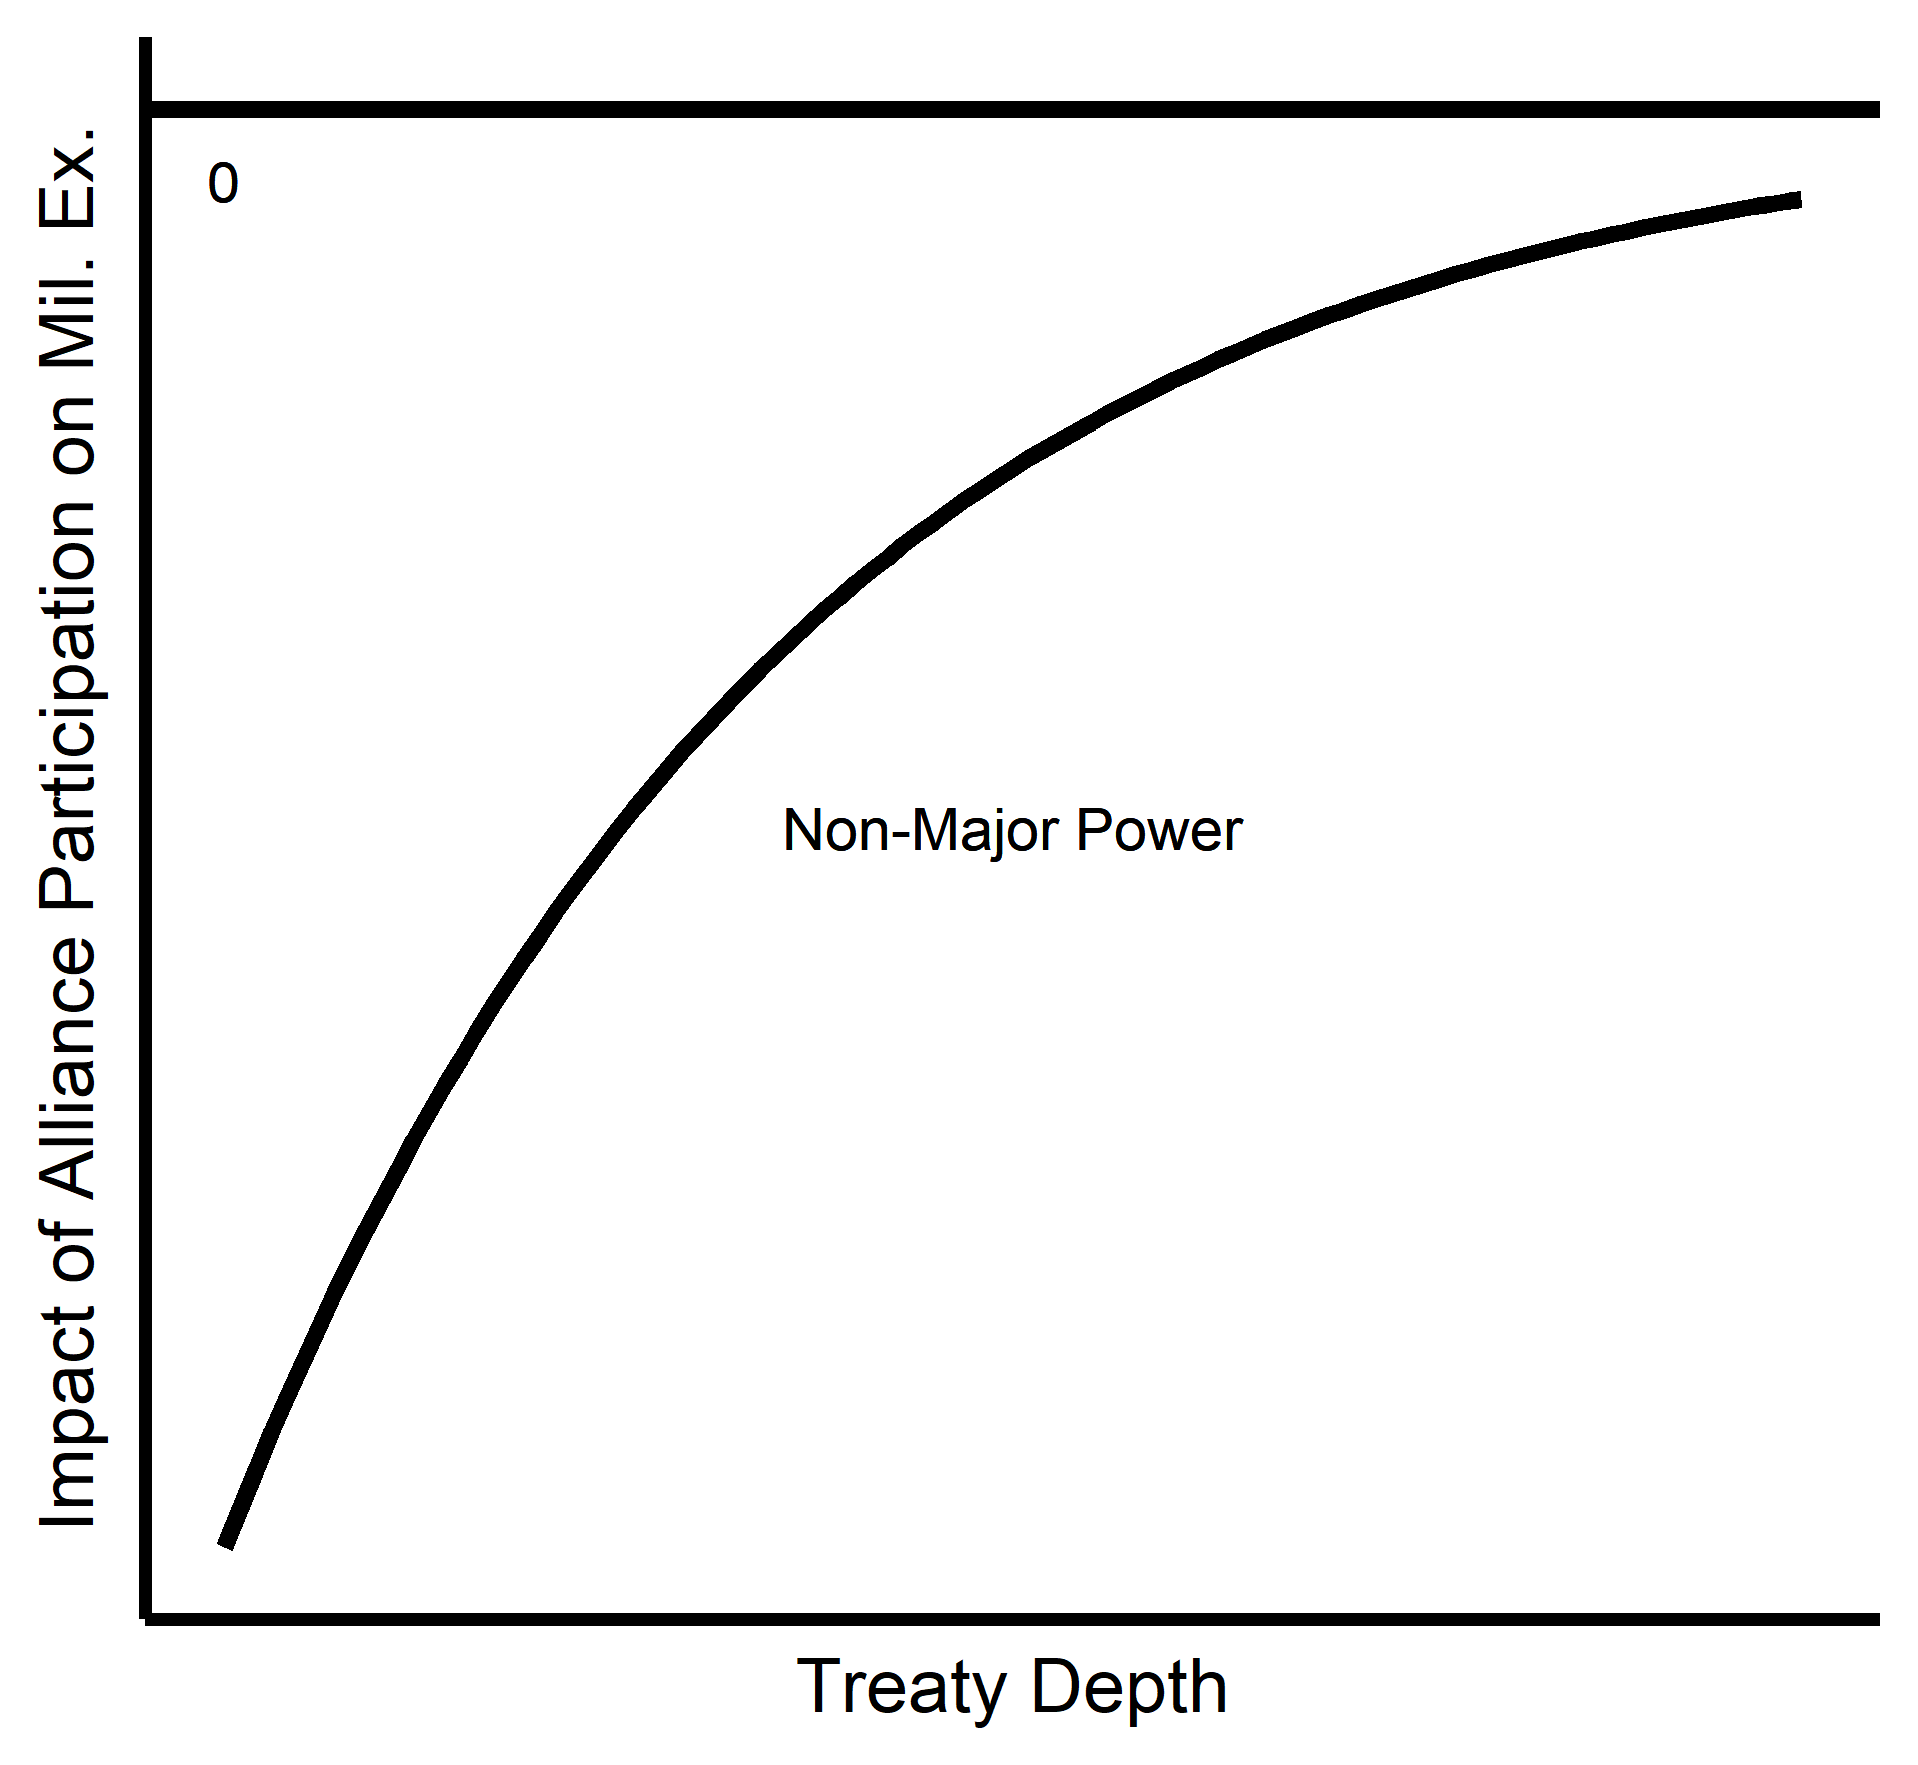
\includegraphics[width=0.95\textwidth]{../figures/illus-arg.png}
	\caption{Abstract illustration of the link between treaty scope and the impact of alliance participation on military spending.
	The top curve represents the impact of alliance participation on growth in major power military spending across the range of treaty scope.
	The bottom curve plots the same function for non-major powers.}
	\label{fig:illus-arg}
\end{figure}


\autoref{fig:illus-arg} illustrates my claims about military spending by plotting a hypothetical link between treaty scope and the impact of alliance participation on military spending. 
The top curve shows a possible relationship for major powers, while the bottom curve tracks the same association for non-major powers. 
The symmetry, shape and levels of the curves are not essential to the argument.
\autoref{fig:illus-arg} only shows the need to be careful moving from changes in spending growth to changes in levels. 


For major powers, lower military expenditure growth as treaty scope increases could still produce higher spending levels. 
Greater treaty scope reduces the positive correlation between treaty participation and military spending among major powers. 
Even a broad treaty may lead to positive growth in military spending. 


For non-major powers, higher growth in spending in a broad treaty scope could remain negative. 
Broad treaties attenuate the negative correlation between alliance participation and military spending in non-major powers. 
But so long as growth from alliance participation remains negative, the level of military spending will fall. 


% Transition para
Because my argument focuses on differences between broad and narrow treaties, the research design must measure alliance treaty scope and compare alliances.  
I use a measurement model to infer treaty scope from formal content, then connect alliances to military spending with a multilevel model. 
The next section describes the research design in more detail. 



\section{Research Design} 


% two contributions: Develop latent str. measure and then put it into an ML model
The research design makes two contributions. 
First, I develop a latent measure of alliance treaty scope. 
Second, I employ that measure in a multilevel model, connecting alliance-level variation with state-level outcomes. 
To examine differences between major and non-major powers, I estimate the multilevel model in separate samples of major and non-major powers from 1816 to 2007. 
The next section describes the measure of alliance treaty scope. 


\subsection{Measuring Alliance Treaty Scope} 


% Intuituion behind latent measures: observed char reflects underlying concept
Observed alliance promises reflect the underlying scope of the treaty. 
Broad treaties contain more costly commitments. 
Therefore, I use observed alliance characteristics to infer treaty scope.


Using observed treaty conditions as indicators of underlying scope could produce two measures. 
One possible measure is an additive index of treaty scope, where treaties with multiple costly promises have higher index values. 
This assumes each indicator is equally important, which is unlikely. 
Instead, I employ latent variable modeling, which is a more flexible way to use observable characteristics to infer an underlying trait.  
The measurement model estimates the correlations between alliance treaty content and the underlying formal scope to predict the scope of each treaty. 


% Justify use
Measurement models have a rich history in political science.\footnote{\cite{Clintonetal2004, TreierJackman2008, Fariss2014}}
Benson and Clinton use a mixed factor analysis model to measure alliance scope, depth and capability.\footnote{\cite{BensonClinton2016, Quinn2004}} 
I emulate Benson and Clinton's approach, but employ more indicators of scope and a better estimator. 


% How the model works
I use a Bayesian Gaussian Copula Factor Model\footnote{\cite{Murrayetal2013}} to measure alliance treaty scope. 
Murray et al's model improves inferences from mixed factor analysis for continuous, ordinal, and binary observed data by relaxing distributional assumptions. 
Given discrete observed variables and non-Gaussian latent variables, the dependence among the latent variables and their marginal distributions are both influenced by the latent variables.
This model breaks the dependence between the latent factors and marginal distributions by using copulas to encode the dependence among the latent variables.\footnote{Copulas are a distribution function on $[0, 1]^p$ where each univariate marginal distribution is uniform on [0, 1].}


Beyond the semiparametric aspect, this measurement model is a standard mixed factor analysis.
Factor analysis estimates the association between observed variables and some latent factor.
Each observed variable has a factor loading--- the association between the observed variable and the latent variable.  
Like standardized regression coefficients, factor loadings range from -1 to 1, so observed variables are positively or negatively correlated with the latent factor.  
For each observation, a linear combination of observed alliance characteristics predicts latent treaty scope, like a regression with an unobserved outcome.  


I estimated the model using observed data from all 745 alliances in the alliance-level ATOP data.\footnote{\cite{Leedsetal2002}}
Indicators of treaty scope are divided between the potential costs of abrogation and additional cooperation.
The potential costs depend on promises of defensive support, offensive support, neutrality, consultation, non-aggression and unconditional military support. 
Extra cooperation includes military aid, economic aid, bases, international organization formation, integrated military command, as well as promises to form new agreements in multiple issue areas and to forgo competing alliances. 
The argument suggests there is a single latent factor underlying variation in all 13 indicators, so I fit the model with one latent factor. 


I used Parameter expanded Gibbs sampling, the default generalized double Pareto (GDP) prior, 10,000 burn-in iterations of the MCMC chain, and 20,000 samples thinned every 20 observations to ensure convergence. 
The estimates include posterior distributions for the factor loadings and the latent factor. 
Because treaty scope is the quantity of interest, I focus on the posteriors of the latent factor. 


% Show the measure for all alliances- note I'll only focus on treaties w/ military support.
Each alliance has a unique posterior distribution of its latent scope. 
I use the mean of that posterior to measure treaty scope. 
\autoref{fig:ls-summary} describes the latent measure for ATOP alliances with defensive or offensive commitments from 1815 to 2016.
I examine the 289 alliances with military support because prior studies of alliance participation and military spending emphasize these treaties.\footnote{
I estimated the measurement model on all alliances, including those without military support to capture the contributions of military support to treaty scope.}
The posterior mean captures the expected scope of an alliance treaty, conditional on the formal promises it makes. 


There is substantial variation in the scope of alliance treaties. 
The top panel of \autoref{fig:ls-summary} is a histogram of mean treaty scope for alliances promising military support.  
Most treaties are concentrated between .5 and 1.5 on the latent scale, but approximately 40 treaties fall outside this range. 
The bottom panel of \autoref{fig:ls-summary} plots the posterior means and uncertainty in those estimates against the start year of the treaty. 
Even after accounting for uncertainty, it is possible to distinguish between some alliances. 


\begin{figure}
	\centering
		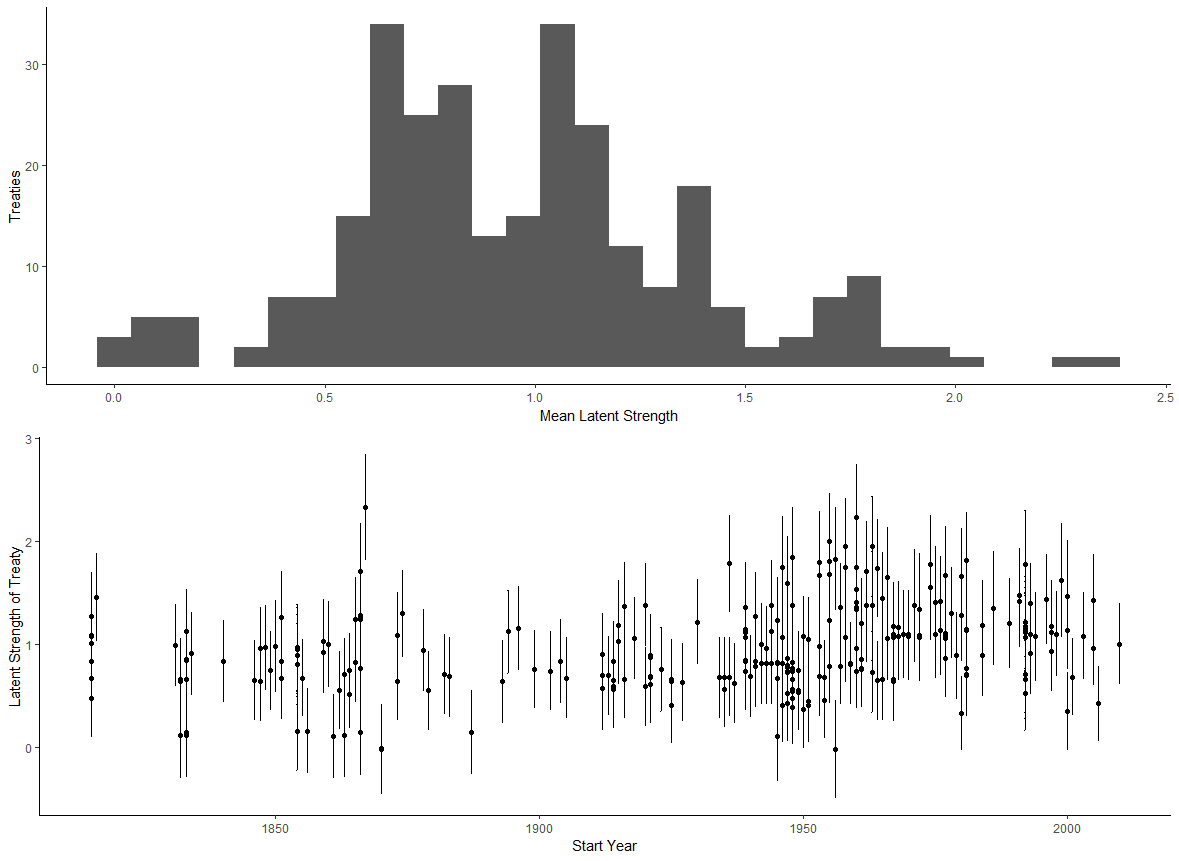
\includegraphics[width=0.95\textwidth]{../figures/ls-summary.png}
	\caption{Summary of latent measure of alliance treaty scope for 289 alliances promising military support from 1816 to 2016. The top panel is a histogram of the expected of alliance treaty scope. The bottom panel plots mean treaty scope (points) and the standard deviation (error bars) against the start year of the treaty.}
	\label{fig:ls-summary}
\end{figure}


% Cases- especially broad and narrow treaties
Although the values of the latent measure are not intrinsically meaningful, differences between treaties on the latent scale are informative. 
The mean of treaty scope is 0.92, and the median is 0.90. 
The median treaty is an 1854 agreement between Austria, France, and Britain against Russia in the Crimean war (ATOP ID 1180). 
The most narrow treaty is an 1870 neutrality and offense pact between France and Britain (ATOPID 1300), which Britain used to protect Belgian neutrality during the Franco-Prussian war.  
Britain formed an identical alliance with Prussia in 1870, which scores nearly the same on the latent measure.\footnote{
Sampling variation produces small differences in the scores.} 
Both treaties have only offensive and neutrality promises, conditional on France and Prussia respecting Belgian neutrality, making them quite narrow. 


NATO (ATOPID 3180) has a mean latent scope of 0.73, placing it in the second quartile of military alliances. 
NATO's two costly provisions are the defense obligations in Article 5 and establishing the Atlantic Council. 
According to the ATOP coding sheet for NATO, ``There are numerous bilateral agreements among NATO members re: military aid, bases, etc. but they do not qualify as separate alliances, nor are they part of the overall NATO structure.''
The NATO treaty is below average in formal scope in part because additional commitments fall outside the formal treaty.    


The three broadest treaties are an 1867 alliance between Prussia and Hesse (ATOPID 1290), a 1955 treaty between Greece, Turkey and Cyprus (ATOPID 3400) and the United Arab Republic (ATOPID 3300).  
All these alliances supplement promises of military support with other costly cooperation. 
The Prussia--Hessian treaty formed on the eve of war with Austria and includes military aid, integrated military command and basing agreements in addition to offensive and defensive promises. 
The United Arab Republic attempted to unify Syria and Egypt, so it commits to defense, integrated military command, military aid, multiple international organizations, and basing rights. 
In the alliance between Greece, Turkey, and Cyprus, Greece and Turkey set up military aid, an integrated command and international organizations to mange relations on the island.
These extra commitments made arrangements between historic enemies in Cyprus more credible. 
The UAR and Greco-Turkish treaties were undone by domestic coups in Turkey and Syria, but that does not diminish the breadth of cooperation they sought. 


The latent measure has some face, concept, and discriminant validity. 
For face validity, the UAR is a broader commitment than a promise to respect Belgian neutrality. 
The most narrow treaties make few costly promises beyond military support, matching my conceptualization of treaty scope. 
Last, this measure can distinguish between broad and narrow commitments. 


My argument uses variation in treaty scope between alliances to explain growth in military spending.
Differences in scope at the alliance level modify the impact of alliance participation on growth in military spending at the state-year level. 
Therefore I use a multilevel model to estimate the association between treaty scope and military spending.  
The next section summarizes the multilevel model. 


\subsection{Multilevel Model} 


% Best fit for theoretical process. Can compare alliances. 
Multilevel modeling is a natural way to bridge levels of analysis.
My model estimates heterogeneous effects of alliance participation on military spending and uses treaty characteristics to explain variation across alliances. 
I can simultaneously make inferences about the specific impact of individual treaties and the general role of treaty characteristics like scope. 
To facilitate computation and interpretation, I fit the model using Bayesian estimation in STAN.\footnote{\cite{Carpenteretal2016}. See the appendix for details of the weakly informative prior distributions and evidence the chains converged.}


This research design adds complexity to a traditional panel data model. 
But the additional components generate novel inferences to connect the argument and research design. 
The hypotheses emphasize differences in treaty scope, so the model contains a corresponding coefficient.


Most panel models use a state-level proxy for alliance characteristics, which compares states rather than alliances.
Aggregating scope at the state-year level of analysis may produce misleading inferences.\footnote{\cite{McElreath2016}}
Multilevel modeling retains the structure of the data, where states are members of multiple alliances. 
Connecting the alliance and state level of analysis generates inferences of alliance-level variation impacts annual growth in state military expenditures. 


Besides connecting alliance and state level variation, the multilevel model generates novel comparisons between alliances by estimating the specific impact of each alliance on members' military expenditures. 
Partial pooling of these alliance-specific parameters generates reasonable estimates for every treaty, which can be used to compare treaties. 
The next section details the model specification. 
 


\subsubsection{Model Specification} 

% Two separate but connected regressions
% State-level regression- alliances enter through spending matrix.
This multilevel model connects two distinct regressions. 
The base is a state-year-level regression, which is similar to a random effects panel data regression.
A second alliance-level regression modifies parameters in the first regression, like an interaction. 


The state-year-level regression starts with a distribution for the outcome:
\begin{equation}
y \sim student_t(\nu, \mu, \sigma)
\end{equation}
 

$y$ is the dependent variable--- growth in military spending. 
I model spending growth using a t-distribution with degrees of freedom $\nu$ to address heavy tails.\footnote{I estimate $\nu$ directly.}
$\sigma$ is analogous to the error term in a frequentist regression--- this captures unexplained variation in spending growth.  
$\mu$, the mean of the outcome, depends on several factors.
\begin{equation}
\mu = \alpha + \alpha^{st} + \alpha^{yr} +\textbf{W}_{n \times k} \gamma_{k \times 1}  + \textbf{Z}_{n \times a} \lambda_{a \times 1} 
\end{equation}


Growth in spending is a function of an overall intercept $\alpha$, state and year varying intercepts $\alpha^{st}$ and $\alpha^{yr}$ and a matrix of state-level control variables $\textbf{W}$.
These components comprise a standard random effects model. 
The $\textbf{Z} \lambda$ term incorporates alliance participation.


$\textbf{Z}$ is a matrix of state participation in alliances. 
Columns correspond to each of the $a$ alliances in the data, and rows to state-year observations. 
If a state is not in the alliance, the corresponding cell of the matrix is zero.
If a state is part of the alliance in a given year, the matrix element contains the log of total allied military spending.


I use total allied spending in the alliance participation matrix because more capable alliances provide extra benefits.
Increasing allied capability makes promises of military support more valuable.\footnote{\cite{Johnsonetal2015}} 
$\textbf{Z}$ encodes a quasi-spatial indicator of alliance participation for all $a$ alliances in the data. 
States can be members of multiple treaties at once, so observations are not neatly nested. 
This specification allows each alliance to have a unique impact on military spending as states participate in multiple treaties. 


$\lambda$ is a vector of parameters which estimate the impact of participation in specific alliances on military spending. 
Because the non-zero elements of $Z$ are allied spending, the $\lambda$ parameters capture alliance members' responsiveness to allied capability. 
Each alliance has a unique $\lambda$. 
The $\lambda$ parameters have shared distribution, so I assume alliances are similar but different in how they impact growth in military spending. 


% Alliance-level regression:
The second part of the multilevel model uses alliance characteristics to predict how alliance participation is associated with growth in military spending. 
The $\lambda$ parameters are the outcome in an alliance-level regression.
As a result, the impact of alliance participation on members' military spending depends on treaty characteristics, including scope. 
In this second-level regression: 


\begin{equation}
\lambda_{a} \sim N(\theta_{a}, \sigma_{all})
\end{equation} 
and 
\begin{equation}
\theta_{a} = \alpha_{all} + \beta_1 \mbox{treaty scope} + \textbf{X}_{a \times l} \beta
\end{equation}


% Like an interaction between alliance and state-level factors 
In the alliance-level regression, $\textbf{X}$ is a matrix of the $l$ alliance-level control variables and $\alpha_{all}$ is the constant.
Adding $\sigma_{all}$ means predictions of $\lambda$ are not deterministic--- the alliance level regression contains an error term. 
A larger $\sigma_{all}$ indicates more variation in how alliance participation impacts military spending. 
The second-level regression includes treaty scope, and each $\beta$ parameter modifies the impact of alliance participation on growth in military spending. 
The $\beta$s are like marginal effects in an interaction. 


Treaty scope impacts military spending by changing the consequences of alliance participation. 
Changing treaty scope shifts $\lambda$, which in turn affects growth in military spending.
Hypothesis 1 predicts $\beta_1$ will be negative among major powers, and Hypothesis 2 expects $\beta_1$ will be positive for non-major powers.
$\beta_1$ compares broad and narrow treaties in each sample. 


% Provide an example observation
Consider one observation as an example of how the model works. 
Growth in Argentina's military spending in 1955 depends on Argentina's economic growth, political regime, conflict participation, and rival military spending. 
Argentine participation in the Rio Pact and OAS also changes growth in spending through allied capability. 


\begin{equation}
\begin{split}
& \mbox{Argentina 1955} = \mbox{Overall mean}
+ \mbox{Argentine Intercept} + \mbox{1955 Intercept} 
+ \mbox{Argentine Characteristics} \\
& + \lambda_{OAS} * \mbox{OAS Expenditure} + \lambda_{Rio} * \mbox{Rio Pact Expenditure}
\end{split} 
\end{equation}


$\lambda_{OAS}$ and $\lambda_{Rio}$ capture the impact of participating in each alliance and are a function of the alliance level regression. 
Characteristics of the OAS and Rio Pact alter their respective $\lambda$ parameters.
Other alliances have no impact on growth in Argentine military spending. 


In this model, the $\beta$ parameters capture the general association between key alliance characteristics and military spending. 
The $\lambda$ parameters express the impact of participation in each alliance, permitting heterogeneous effects of different treaties. 
Using alliance characteristics to modify the impact of alliance participation matches my conditional argument. 
I now describe the sample and covariates in the analysis.  



\subsection{Sample and Covariates} 

% Sample of states 
I estimate this model on two samples of states from 1816 to 2007--- one sample of major powers, the other of non-major powers. 
Splitting the sample means I cannot directly compare estimates from the major and non-major power samples, but I can show different trends in the two samples. 
A split sample followed by graphical comparison of the estimates approximates letting the slopes vary.\footnote{See \citet{GelmanHill2007}. I also estimated a varying slopes model, which generates similar inferences about treaty scope. More information on that model and the results is available in the appendix.}
If major powers focus on influence and non-major powers emphasize immediate territorial security, alliance-level coefficients besides strength will vary between major and minor powers.
Splitting the sample is a simple way to capture these distinctions. 


% sample of alliances: restricted to treaties with military support
I classify state-year observations using a measure of major power status from the Correlates of War Project. 
As with the argument, this is a course division, but it matches the sharp comparison in the argument and employs a widely used measure. 
Alliance participation data comes from the ATOP project.\footnote{\cite{Leedsetal2002}} 
I focus on participation in defensive and offensive treaties, because prior studies of alliances and military spending examine these treaties. 


The non-major power sample contains 8,668 observations in the state-level regression, and 192 alliances. 
There are 930 major power observations and 148 alliances. 
Although the major power sample is smaller and has fewer states, Bayesian estimation should generate plausible results.\footnote{\cite{Stegmueller2013}} 


% DV: growth in milex
The state-year dependent variable is growth in military spending.
Growth in military expenditures is calculated as:
\begin{equation}
\mbox{Growth Mil. Expend} = \frac{ \mbox{Change Mil. Expend}_t }{ \mbox{Mil. Expend}_{t-1} }
\end{equation} 
I used the Correlates of War Project's data on military spending to measure growth.\footnote{\cite{SingerCINC1988}} 
Growth in spending is equal to changes in spending as a share of the previous year's military spending, so changes are relative to previous levels of spending. 


Using military expenditure growth as the dependent variable helps the research design. 
The level of military spending is not stationary for most states, especially in longer panels. 
Thus, using growth in spending reduces the risk of spurious inferences.
Benchmarking changes to prior expenditures also facilitates comparisons across states and over time. 


% key IV: mean treaty scope
The key independent variable is the mean latent scope of each alliance. 
This variable enters the model in the alliance-level regression. 
I also include a series of state and alliance-level controls. 


% Describe covariates at each level. 
In the state-level regression, I adjust for several variables that are correlated with alliance participation and military spending. 
State-level covariates include GDP growth,\footnote{\cite{Boltetal2018}} regime type, international war,\footnote{\cite{Reiteretal2016}} civil war participation,\footnote{\cite{SarkeesWayman2010}} annual MIDs,\footnote{\cite{Gibleretal2016}} rival military spending,\footnote{\cite{ThompsonDreyer2012}} and a dummy for Cold War years.
Conflict participation, alliances, and military spending are all correlated.\footnote{\cite{SeneseVasquez2008}}
I include growth in GDP instead of levels of GDP because GDP levels are non-stationary, and economic growth shapes the opportunity costs of military spending.\footnote{\cite{Kimball2010, Zielinskietal2017}} 


The alliance-level regression contains the mean of the latent treaty scope--- the key independent variable. 
Other alliance level variables are correlates of treaty design and military spending, including the number of members and share of democracies in a treaty at time of formation.\footnote{\cite{Chibaetal2015}} 
I adjust for superpower membership--- whether the United States or Soviet Union participated in a treaty during the Cold War. 
Two dummy indicators of wartime alliances and asymmetric obligations\footnote{\cite{Leedsetal2002}} complete the alliance-level regression specification. 


Adjusting for all of these covariates helps address systemic differences between states and alliances from strategic selection into alliances. 
Regime type and external threat are especially important in that endeavor. 
The next section describes the results from the major and non-major samples.
 

\section{Results}


Results are based on 2,000 total samples from four chains, with 1,000 warm-up iterations. 
To facilitate model fitting, I employed a non-centered parameterization of the varying intercepts and a sparse matrix representation of \textbf{Z}. 
Standard convergence diagnostics indicate the chains adequately explored the posterior density.\footnote{See the appendix for more details on convergence.} 


% note on interpreting Bayesian results
Because I use Bayesian modeling to estimate the association between treaty scope and growth in military spending, each coefficient has a posterior distribution--- the likely values of the coefficient conditional on the priors and observed data.
There are no indicators of statistical significance. 
Instead I calculate the negative and positive posterior probability for the two treaty scope coefficients to assess Hypotheses 1 and 2.


% show latent strength coefficient in each subset of data
\begin{figure}[htbp]
	\centering
		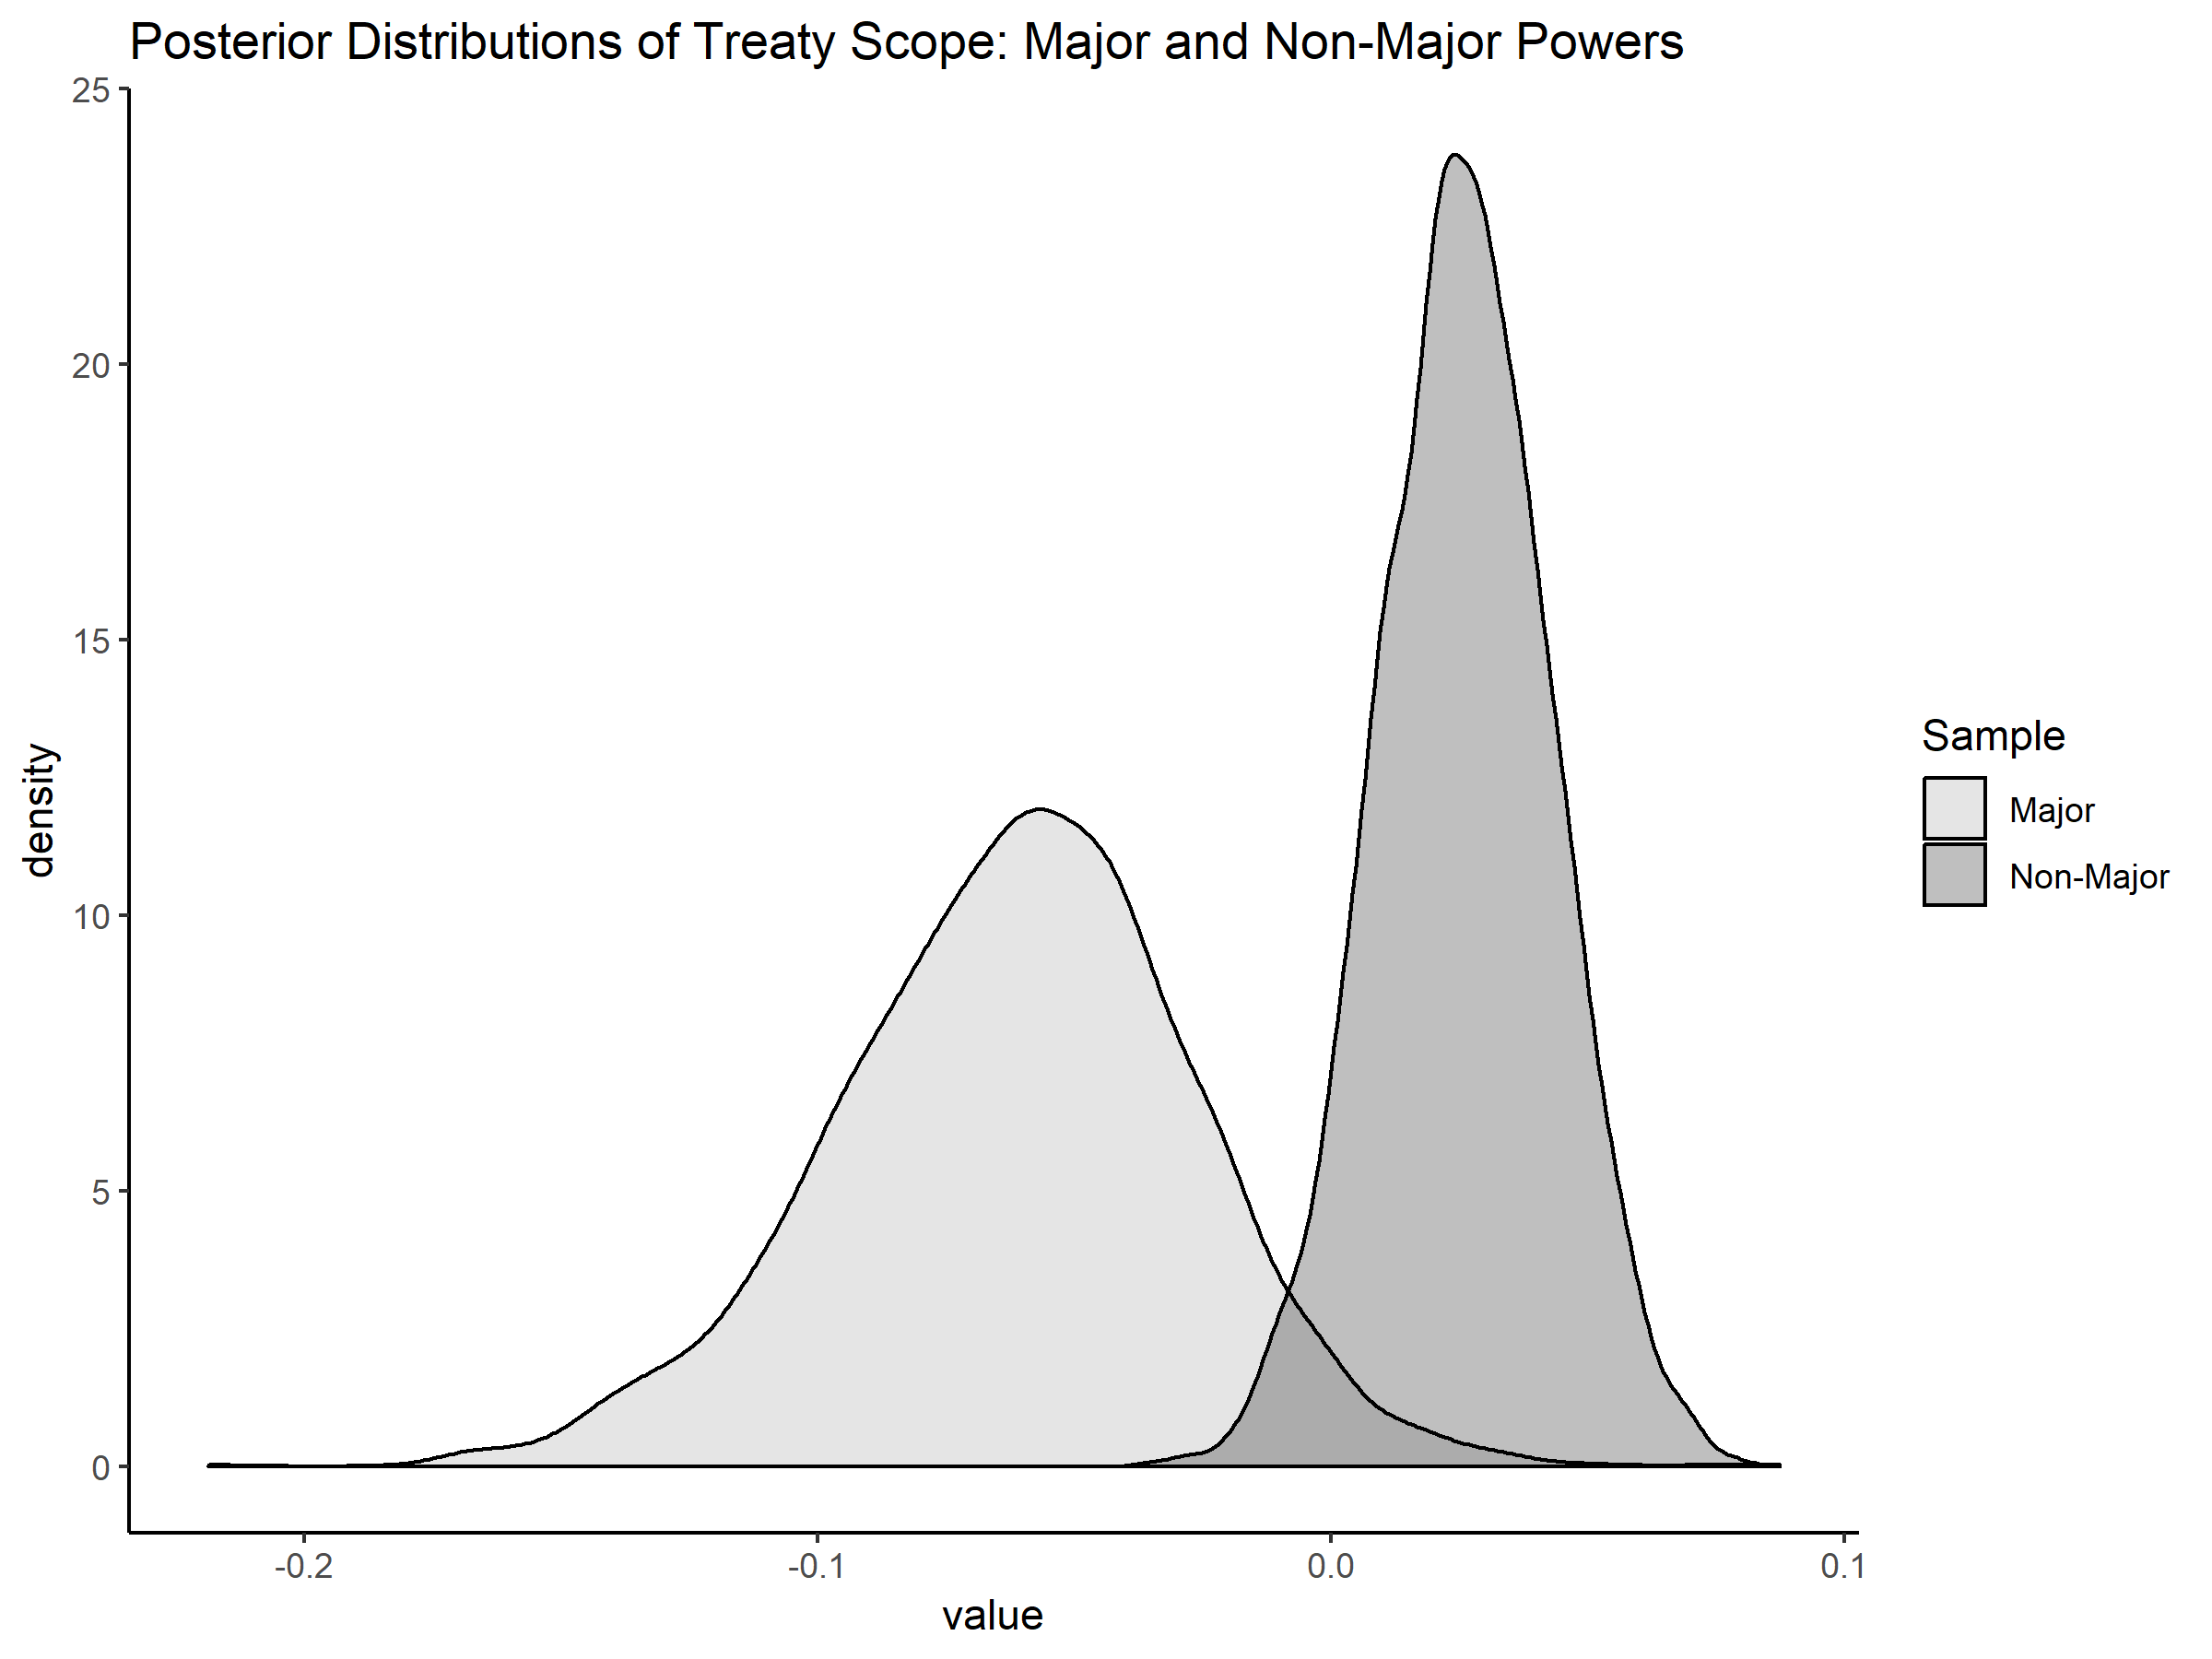
\includegraphics[width=0.95\textwidth]{../figures/scope-dens-split.png}
	\caption{Posterior density of association between alliance treaty scope and growth in military spending among major and non-major powers, 1816 to 2007. 96\% of the major power posterior mass is negative. 94\% of the non-major power posterior mass is positive.}
	\label{fig:str-dens}
\end{figure}


\autoref{fig:str-dens} plots the full posterior density of the treaty scope coefficients in the major and minor power samples.\footnote{The smaller major power sample increases variance in all the coefficient estimates.} 
96\% of the posterior mass for major powers is negative. 
94\% of the posterior mass for minor powers is positive. 


The preponderance of evidence matches the predictions of Hypotheses 1 and 2. 
For major powers, there is a 96\% chance treaty scope is negatively associated with growth in military spending. 
There is a 94\% chance treaty scope is positively associated with growth in military spending for non-major powers.


Though the two coefficients have the expected sign, more evidence is needed to establish substantive importance. 
To assess the substantive impact of a change in treaty scope, I compare the expected value of the coefficient to typical growth in military spending in each sample. 
Among major powers, the mean of the treaty scope coefficient is -0.05, and median growth in military expenditures is 0.04.\footnote{The median is a better summary of the dependent variable because large positive and negative outliers influence the mean.} 
So a one-unit increase in treaty scope more than offsets the typical annual growth in military spending. 
This change in spending is a plausible effect--- 5.1\% of the 2018 US defense budget was spent directly on NATO.\footnote{See the following IISS blog post: https://www.iiss.org/blogs/military-balance/2018/07/us-and-nato-allies-costs-and-value.} 


For non-major powers, the mean of the treaty scope coefficient is 0.03, and median growth in military expenditures is 0.06. 
Greater treaty scope increases growth in minor power military expenditures by about half of typical growth. 
In both the major and non-major power samples, the expected impact of higher treaty scope has a meaningful substantive effect.\footnote{Of course, uncertainty in the posterior estimates includes larger and smaller effects.}


I also assess substantive importance by looking at patterns in the $\lambda$ parameters. 
Each $\lambda$ measures the impact of treaty participation. 
If treaty scope has a large influence on alliance participation, it will appear in the $\lambda$ estimates. 
There should be a negative trend in the expected value of $\lambda$ as treaty scope increases in major power alliances and a positive trend among non-major power alliances. 


\begin{figure}[htbp]
	\centering
		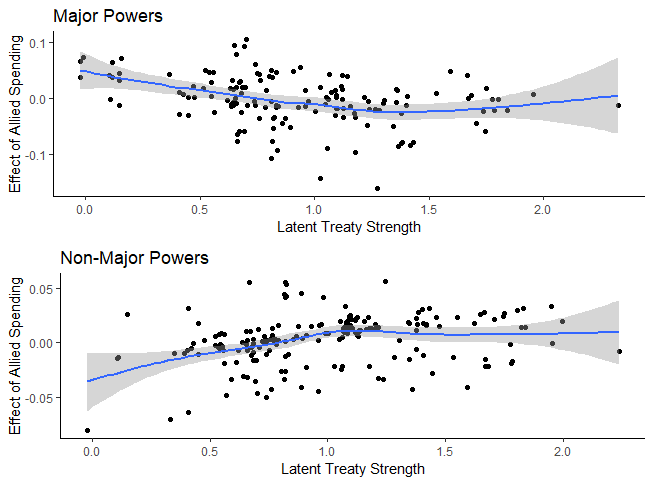
\includegraphics[width=0.95\textwidth]{../figures/lambda-ls-scatter.png}
	\caption{Scatter plots of trends in mean $\lambda$ parameters and treaty scope. $\lambda$ is the total impact of alliance participation on growth in military spending. The top panel is major powers, where this is a negative trend between $\lambda$ and treaty scope. In the bottom panel the same trend is positive for non-major powers. Trend lines estimated using linear regression.}
	\label{fig:lambda-ls-scatter}
\end{figure}


\autoref{fig:lambda-ls-scatter} plots the expected value of $\lambda$ across the range of treaty scope in the two samples. 
In the major power sample, there is a negative trend in the scatter plot.
For non-major powers, the trend is positive.
The correlation between mean $\lambda$ and treaty scope is statistically significant in both samples. 


These trends match the underlying logic of Hypotheses 1 and 2. 
Limited treaties tend to increase growth in defense spending for major powers, but that positive association falls as treaty scope increases. 
Narrow treaties often reduce growth in military spending among non-major powers, while most broad treaties have a less negative effect. 
Because other treaty characteristics and unmeasured factors also influence the $\lambda$ estimates, neither trend is deterministic. 


Trends in the $\lambda$ parameters across the range of treaty scope suggest that treaty scope has a substantial impact. 
Even after accounting for other alliance characteristics, alliance scope drives the impact of alliance participation down for major powers, and up for non-major powers. 
Treaty scope is a key source of heterogeneity in how alliance participation impacts military spending. 


While the statistical model estimates general associations, it does not show the underlying process. 
To further illustrate the argument, I offer a brief description of US alliance politics.   
I focus on NATO--- the most important alliance in the international system.  


\subsection{NATO Treaty Scope and Military Spending}


% add something on estimates from ML model
The multilevel model includes estimates of the specific impact of treaty participation, including for NATO. 
In the major power sample, NATO membership adds 0.04 to growth in military spending in expectation.
For non-major powers, NATO membership lowers growth in military expenditure by -0.006 in expectation.\footnote{
The UK and France are major powers from 1945 on, and Germany is a major power after 1991. Therefore, these estimates may understate reduced growth in spending by NATO members, because all three of these states relied on US capability for protection. Positive growth in major power spending is driven by the United States.}
This is because NATO's formal promises are weaker than average among defense treaties. 


% generally limited treaties 
American choices in treaty design had important consequences for junior partners and reassurance. 
While forming NATO, the United States balanced between fear of ``foreign entanglements'' and maintaining influence to check the USSR.
The Soviet threat led US policymakers to form several alliances, but domestic opposition weakened the formal promises in most treaties. 


% NATO 
Limited formal commitments in NATO led to additional defense outlays to support Washington's influence.
Despite concern about Soviet intentions, isolationists in the US Senate feared an alliance would force America to intervene automatically if partners were attacked, bypassing the power of Congress to declare war.\footnote{\citet[pg. 280-1]{Acheson1969}}
Thus, Article V states that if one member is attacked the others ``will assist the Party or Parties so attacked by taking forthwith, individually and in concert with the other Parties, \emph{such action as it deems necessary}'' (emphasis mine). 
Military support was and is not guaranteed. 


The absence of automatic US involvement increased demand for reassurance by European allies. 
Europeans feared that if the Soviets invaded, the United States would decide not to fight. 
Bilateral agreements on troop deployments then became a means of reassurance. 


In 1950 West Germany formally requested clarification on whether an attack on US forces in Germany would be treated as an armed attack on the United States. 
US officials said it would, thereby providing a crucial assurance.\footnote{\citet[pg. 395]{Acheson1969}} 
A 1951 presentation by Dean Acheson to Dwight Eisenhower argued European allies ``fear the inconstancy of United States purpose in Europe. ... These European fears and apprehensions can only be overcome if we make the necessary full and active contribution in terms of both military forces and economic aid.''\footnote{\citet[pg. 3]{Acheson1951}}
After agreeing to deploy troops, US policymakers hoped Europeans would soon provide more for their own defense, while acknowledging the United States ``should not dictate what they shall do.''\footnote{\citet[pg. 2]{Johnson1950}} 


Though the executive branch sought a broad NATO treaty, isolationist fears of foreign entanglement constrained its formal scope. 
Senate opposition to military aid\footnote{\citet[pg 285]{Acheson1969}} resulted in bilateral arrangements and aid through other channels. 
Due to limited formal scope in the NATO treaty, the United States has little leverage on allied military spending. 
NATO members have been free to reduce growth in defense spending. 


In response, American policymakers from Eisenhower to Trump have attempted to browbeat NATO members into spending more. 
These efforts usually fail. 
Most European members of NATO have been unresponsive to changes in external threat and US defense spending.\footnote{\cite{PluemperNeumayer2015}} 


The United States has threatened to leave NATO in response to European ``free-riding,'' but those threats were not credible. 
During the Cold War, US interests in containing the USSR trumped irritation with allied free-riding.  
Without other costly treaty commitments to use as leverage, the United States had few ways to check allied incentives to reduce growth in military spending. 


This brief description of NATO matches the expectations and process of the argument. 
US fear of entanglement led to higher growth in military spending and limited bargaining leverage in alliance maintenance. 
European members gained security and retained the freedom to lower growth in defense spending.   


\section{Discussion}


% Precise interpretation: compares alliances. Not treaty vs absence. 
My findings add to our understanding of alliance participation and military spending and address debates over whether alliance participation increases or decreases military spending. 
Claims alliance participation only increases or decreases military spending are inaccurate. 
Major and non-major powers respond differently to alliance participation because they use treaties for different purposes. 
Moreover, alliance treaty design has distinct ramifications for major and non-major powers. 
Treaty scope decreases growth in major power spending from alliance participation, while increasing non-major power expenditure growth. 


% Link for force multiplier and foreign entanglement
My argument builds on other conditional arguments about alliance participation and military spending\footnote{\cite{DigiuseppePoast2016}} and clarifies where the force multiplier and foreign entanglement perspectives best apply. 
The force multiplier perspective covers non-major powers well. 
But non-major powers cannot reduce growth in military spending in all alliances, because broad treaties constrain their freedom of action.
The foreign entanglement prediction applies to major powers, but broad treaties provide more influence, lowering the positive correlation between alliance participation and growth in military spending. 


This paper connects two previously separate components of the political economy of alliances. 
The first component is work on issue linkage politics in alliances.\footnote{\cite{Mattes2012, Poast2012, Poast2013, Johnson2015}} 
The second is the arms-alliances tradeoff.\footnote{\cite{Morrow1993}}
By using issue linkages to explain when alliance participation increases or decreases military spending, I provide a joint perspective on the political economy of alliances.  


How do the findings compare to prior evidence on alliance participation and military spending? 
Connecting my results with earlier evidence requires renewed attention to specific and general research designs. 
General studies compare states in an alliance to those without one. 
Specific studies estimate responsiveness to allied military spending in a few treaties. 


The results encompass specific and general studies, as I estimate both the impact of individual treaties and general differences between treaties. 
My research design emulates specific studies by estimating the unique impact of participation in individual treaties. 
The alliance-level coefficients compare treaties to capture the general consequences of alliance characteristics. 


% limitations of RD
This paper has several limitations.
First, the argument offers a cursory treatment of the domestic political economy of military spending. 
By reducing domestic politics to an assumption that military spending has opportunity costs, which are decreasing in state size, I elide a rich literature on this topic.\footnote{\cite{WhittenWilliams2011, AlptekinLevine2012}}  
Furthermore, domestic politics shapes how states define their foreign policy interests and the tools they use to pursue those interests.\footnote{\cite{Fordham1998, Fordham2011, Narizny2007}}
At the moment, my argument treats foreign policy interests as given.  


My findings also only address formal issue linkages. 
The measure of treaty strength only includes formal promises, in part because informal issue linkages are hard to observe. 
As a result, my test of treaty scope and the associated issue linkages is probably conservative--- it does not capture phenomena my argument expects should have a similar effect. 


% Strategic treaty design
Strategic alliance design is another possible weakness of the test. 
Non-random selection into different alliances could produce systematic differences between members that are not captured for in my statistical model. 
I attempted to control for correlates of alliance treaty scope, but oversights are possible. 


Despite these limitations, the argument and results provide valuable insights about alliance participation and military spending. 
I explain when alliance participation is associated with more or less growth in military spending, addressing debate between the force multiplier and foreign entanglement views of alliances.  
I provide evidence that how alliance participation impacts military spending depends on state capability and alliance treaty scope using a new measure of alliance treaty scope and a multilevel model. 
The argument and findings have implications for scholars and policymakers. 


\section{Conclusion}

% tie it all together
Alliance participation does not uniformly increase or decrease military spending. 
Both the force multiplier and foreign entanglement views of alliance participation are correct, each in different circumstances.
Alliances are more foreign entanglement for major powers and more force multiplier for non-major powers. 
The exact consequences of alliance participation depend on treaty characteristics, however. 


% Start conclusion
There are several implications of my findings that treaty scope decreases growth in major power military spending from alliance participation, while increasing growth in spending from alliance participation for non-major powers.  
First, they reinforce the importance of accounting for heterogeneity among alliances.
Alliances have heterogeneous effects on many interesting and important outcomes.\footnote{\cite{Leeds2003, Benson2012, DigiuseppePoast2016}} 


% Add paragraph on distributional consequences.
Another implication is the distributional consequences of changes in military spending within states and among alliance members.  
By altering growth in military spending, the design of international alliances alters the domestic political economy of member states. 
The domestic economic consequences of alliance participation are a possible subject for future research. 


% The argument indicates tradeoff
Besides their scholarly value, the argument and evidence help inform policy debates. 
Tradeoffs in alliance treaty design for major and non-major powers can guide our understanding of why some treaties lead to ``free-riding'' and possible policy responses. 
Major powers may be able to check allied free-riding through increasing the scope of their alliance commitments. 
Greater influence requires deeper engagement abroad, however. 


% Implications for policy. 
The United States is currently wrestling with the implications of treaty scope. 
Washington has often decried ``free-riding'' by allies who provide too little for their own defense.\footnote{\cite{Lanoszka2015}} 
But allies are able to free-ride partly because the United States makes limited formal alliance commitments. 
``Foreign entanglements'' may provide more influence to curb falling allied defense spending. 

 
Therefore, growing institutionalization of NATO, including the agreement for all allies to spend at least 2\% of GDP on defense, could help.
More side obligations within NATO tie the United States more closely to Europe, but are a better check on allied free-riding than verbal exhortations. 
Threatening to leave the alliance may not be credible and undermines US gains from alliances. 


The United States could use broad formal commitments as a substitute for greater defense effort in reassuring allies.
Adding scope to treaties may also increase alliance credibility.\footnote{\cite{Poast2013}}
This is not an unconditional call for greater scope in US alliance commitments, however. 
Adjusting existing treaties may be more difficult than designing new alliances. 
The full consequences of treaty scope and attempting to change it require additional scrutiny from scholars and policymakers. 

 



\singlespace
 
\bibliography{../../MasterBibliography} 





\end{document}
